\documentclass[a4paper,12pt,oneside]{ctexbook}
\usepackage{amsmath,amsthm,bm,graphicx,hyperref,mathrsfs,xcolor,titlesec,graphicx}
\title{{{\Huge{\textbf{Physical Waste}}}}\\——各种物理灵感或笔记整理}%textbf用于加粗
\author{猫の薛定谔}
\date{2023年4月1日}
\linespread{1.5}
\newtheorem{theorem}{定理}[section]
\newtheorem{definition}[theorem]{定义}
\newtheorem{lemma}[theorem]{引理}
\newtheorem{corollary}[theorem]{例}
\newtheorem{proposition}[theorem]{命题}
\renewenvironment{proof}{{\it 证明:}\quad}
{\hfill \par}

\titleformat{\section}[block]{\color{black}\Large\bfseries\raggedright}{\thetitle}{1em}{}%通过引入titlesec宏包来修改section的格式,raggedright使其能够左对齐,再引入xcolor宏包还能修改其颜色。\thetitle指令用于编号

\usepackage{fancyhdr}
\pagestyle{fancy}
\cfoot{\thepage}%这条语句可以让页码出现在下方

\begin{document}
	\maketitle
	\pagenumbering{roman}
	\setcounter{page}{1}

	\begin{center}
		\Huge\textbf{前言}
	\end{center}~\

  本文档建立与2023年4月1日,主要用于LaTeX的练习与一些物理笔记的整理。\par 
  时处于愚人节之际,暨Laudau逝世65周年。不知为何,内心甚烦,不知去往何处。\par 
  注:本文档均使用Einstein summation notation!
  \begin{flushright}
  	\begin{tabular}{c}
  		猫の薛定谔\\
  		2023年4月1日
  	\end{tabular}
  \end{flushright}


\newpage
\pagenumbering{Roman}
\setcounter{page}{1}
\tableofcontents
\newpage
\setcounter{page}{1}
\pagenumbering{arabic}

\chapter{NABLA算子}
\section{用抽象指标记号推导Nabla算子相关公式}
%后面可以编写正文
最基本的梯度、散度和旋度均可采用张量表示为\par 
1.$\nabla$$f$=$\partial_a$$f$\par 
2.$\nabla$$\cdot$$\vec{A}$=$\delta_b^a$$\partial_a$$A^b$\par 
3.$\nabla$$\times$$\vec{A}$=$\varepsilon_{ijk}$$\partial_i$$A_j$\par 
\begin{lemma}
	$\varepsilon_{ijk}\varepsilon_{mnk}=\delta_{im}\delta_{jn}-\delta_{in}\delta_{jm}$ 
\end{lemma}
\par 
证明:\textcolor{red}{略}\par 
\textbf{基本内容:}\par
1. $$
\nabla\cdot\left(k\vec{A}\right)=k(\nabla\cdot\vec{A})+\nabla k\cdot\vec{A} 
$$\par 
\begin{proof}
{\color{red}{L.H.S=$\delta_b^a$$\partial_a$$kA_b$=k$\partial_a$$A^a$+$\partial_a$$k$$A^a$=R.H.S}}
\end{proof}
2.$$
\nabla\times(k\vec{A})=k(\nabla\times\vec{A})+\nabla k\times\vec{A} 
$$\par 
\begin{proof}
{\color{red}{L.H.S的第k个分量=k$\varepsilon_{ijk}$}}
\end{proof}


\section{曲面坐标系下的Nabla算子}
对于平面直角坐标系中的一个矢量$\vec{a}=(x,y,z)$,将其变换至球坐标系时,显然有:\par
1.$x=rsin$$\theta$$cos\varphi$\par 
2.$y=rsin$$\theta$$sin\varphi$\par
3.$z=rcos$$\theta$\par
那么对于球坐标系下的单位坐标应该如何用直角坐标来表示呢?
有一点是十分显然的,那就是这两种坐标系的变换对应着一种旋转。如图1.1所示:\par 
\begin{figure}[htpb]
	\centering
	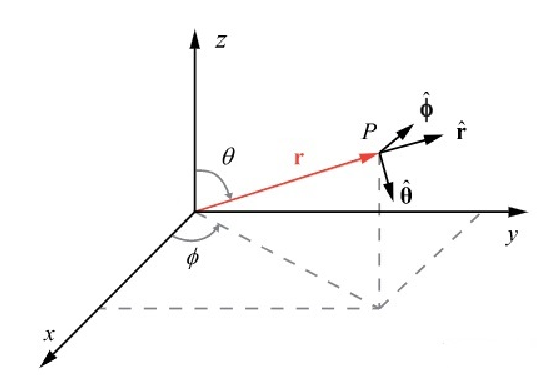
\includegraphics[scale=1]{坐标变换.eps}
	\caption{两种坐标的变换}
	\label{figure}
\end{figure}%上述指令用于调用图片,首先先要将图片转换为eps格式并放入与.tex同一个文件夹中,在输入图片名称即可。htpb分别表示如下含义:h表示当前位置(here),也就是说图片将放在你设置的当前位置,但是如果这一页的空间不足以放下这个图片,此时图片会转到下一页;t顶端(top),此时优先将图片放置在页面的顶部;底部b(bottom)此时优先将图片放置在页面底部; p将图片设置为浮动状态,系统会自动排版图片的位置。一般推荐这几个参数结合使用,比如:[ht]、[htbp],此时这几种位置具有优先级。scale用于修改图片大小。
显然,旋转可分为如下三步:\par
1.以z轴为旋转轴旋转$\varphi$;\par 
2.以y轴为旋转轴旋转$\theta$;\par 
3.最后将($\theta$,r,$\varphi$)转变为(r,$\theta$,$\varphi$).\par
这三步的旋转矩阵分别为:\par 
1.\begin{equation}
	{\textbf{A}= \left[ \begin{array}{ccc}
			cos\phi & sin\phi & 0\\
			-sin\phi & cos\phi & 0\\
			0 & 0 & 1
		\end{array}
    	\right ]}%上面用于输出矩阵
    \nonumber%用于去掉编号
	\end{equation}\par 
2.\begin{equation}
{	\textbf{B}= \left[ \begin{array}{ccc}
		cos\theta & 0 & -sin\theta\\
		0 & 1 & 0\\
		sin\theta & 0 & cos\theta
			\end{array}
	\right ]}\
\nonumber
\end{equation}\par 
3.\begin{equation}
	{\textbf{C}= \left[ \begin{array}{ccc}
			0 & 1 & 0\\
			1 & 0 & 0\\
			0 & 0 & 1
		\end{array}
	\right]}
\nonumber
\end{equation}
所以\par 
	\begin{align}
	 \left(
\begin{array}{c}
	r \\
	\theta \\
	\varphi
\end{array}
\right)&=\textbf{CBA} \left(
\begin{array}{c}
	x\\
	y \\
	z
\end{array}
\right)
\nonumber
\\
    &= \left[ \begin{array}{ccc}
	0 & 1 & 0\\
	1 & 0 & 0\\
	0 & 0 & 1
\end{array}
\right]
\left[ \begin{array}{ccc}
	cos\theta & 0 & -sin\theta\\
	0 & 1 & 0\\
	sin\theta & 0 & cos\theta
\end{array}
\right ]
\left[ \begin{array}{ccc}
	cos\phi & sin\phi & 0\\
	-sin\phi & cos\phi & 0\\
	0 & 0 & 1
\end{array}
\right ]
 \left(
\begin{array}{c}
	x\\
	y \\
	z
\end{array}
\right)
\nonumber
\\
&=\left[ \begin{array}{ccc}
	sin\theta cos\phi & sin\theta sin\phi & cos\theta\\
	cos\theta cos\phi & cos\theta sin\phi & -sin\theta\\
	-sin\varphi & cos\varphi & 0
\end{array}
\right ]
\left(
\begin{array}{c}
	x\\
	y \\
	z
\end{array}
\right)
\nonumber
\end{align}

这样坐标变换就完成了。(樂)\end{document}

